\chapter{Classical and Modern Spectrum Estimation}


\section{Properties of Power Spectral Density}
The proof of equalization has been shown analytically below, starting from equation (9) in the coursework booklet. 
\item
\begin{equation}\label{equ:equation1}
\begin{aligned}
P(\omega ) &= \mathop {\lim }\limits_{N \to \infty } {\rm E}\left\{ {\frac{1}{N}{{\left| {\sum\limits_{n = 0}^{N - 1} {x(n){e^{ - jn\omega }}} } \right|}^2}} \right\}\\
 &= \mathop {\lim }\limits_{N \to \infty } {\rm E}\left\{ {\frac{1}{N}\sum\limits_{{n_1} = 0}^{N - 1} {x({n_1}){e^{ - j{n_1}\omega }}} \sum\limits_{{n_2} = 0}^{N - 1} {{x^*}({n_2}){e^{j{n_2}\omega }}} } \right\}\\
 &= \mathop {\lim }\limits_{N \to \infty } \frac{1}{N}\sum\limits_{{n_1} = 0}^{N - 1} {\sum\limits_{{n_2} = 0}^{N - 1} {{\rm E}\left\{ {x({n_1}){x^*}({n_2})} \right\}} } {e^{j\left( {{n_2} - {n_1}} \right)\omega }}\\
 &= \mathop {\lim }\limits_{N \to \infty } \frac{1}{N}\sum\limits_{{n_1} = 0}^{N - 1} {\sum\limits_{{n_2} = 0}^{N - 1} {{R_{xx}}({n_1},{n_2})} } {e^{j\left( {{n_2} - {n_1}} \right)\omega }}\\
 &= \mathop {\lim }\limits_{N \to \infty } \frac{1}{N}\sum\limits_{{n_1} = 0}^{N - 1} {\sum\limits_{{n_2} = 0}^{N - 1} {{R_{xx}}({n_1} - {n_2})} } {e^{j\left( {{n_2} - {n_1}} \right)\omega }}
\end{aligned}
\end{equation}
In equation \ref{equ:equation1}, ${R_{xx}}({n_1},{n_2})$ is the auto-correlation between $x(n_1)$ and  its complex conjugate $x(n_1)$. The two summations can be converted into one summation by representing $n_1-n_2$ as $\tau$ and the the range of $\tau$ is $[-(N-1),N-1]$. 
According to the rule that 
\begin{equation}
\sum\limits_{{n_1} =  - N}^N {\sum\limits_{{n_2} =  - N}^N {{R_{xx}}(k)} } {e^{jk\omega }} = \sum\limits_{k =  - 2N}^{2N} {(2N + 1 - \left| k \right|} ){R_{xx}}(k){e^{jk\omega }}
\end{equation}
We get \ref{equ:equation2},
\begin{equation}\label{equ:equation2}
\begin{aligned}
P(\omega ) &= \mathop {\lim }\limits_{N \to \infty } \frac{1}{N}\sum\limits_{k =  - (N - 1)}^{N - 1} {(N - 1 + 1 - \left| k \right|){R_{xx}}(k){e^{j\omega k}}} \\
 &= \mathop {\lim }\limits_{N \to \infty } \sum\limits_{k =  - (N - 1)}^{N - 1} {{R_{xx}}(k){e^{j\omega k}}}  - \mathop {\lim }\limits_{N \to \infty } \frac{1}{N}\sum\limits_{k =  - (N - 1)}^{N - 1} {\left| k \right|{R_{xx}}(k){e^{j\omega k}}} \\
 &=\sum\limits_{k =  - \infty }^\infty  {{R_{xx}}(k){e^{j\omega k}}}  - \mathop {\lim }\limits_{N \to \infty } \frac{1}{N}\sum\limits_{k =  - (N - 1)}^{N - 1} {\left| k \right|{R_{xx}}(k){e^{j\omega k}}} 
\end{aligned}
\end{equation}
Under a mild assumption that the co-variance sequence ${R_{xx}}(k)$ decays rapidly, which is shown in \ref{equ:equation3},
\begin{equation}\label{equ:equation3}
\mathop {\lim }\limits_{N \to \infty } \frac{1}{N}\sum\limits_{k =  - (N - 1)}^{N - 1} P(\omega ) = {\left| k \right|{R_{xx}}(k){e^{j\omega k}}}=0
\end{equation}
And under this assumption, \ref{equ:equation2} can be written as the DTFT of the Autocovariance Function (ACF) as expressed as in \ref{equ:equation4}. It is also defined as Power Spectral Density (PSD). 
\begin{equation}\label{equ:equation4}
P(\omega ) &= \sum\limits_{k =  - \infty }^\infty  {r(k){e^{-j\omega k}}} 
\end{equation}
%
\section{Periodogram-based Methods Applied to Real–World Data}
%% a)
a) The figure \ref{fig:1_2_a} shows original sunspot time series and the the Hamming-window periodogram of the series. The three plots represent the raw data(blue), the centered and detrended data(orange), and the logarithmic data(yellow). 
It is known that the original data have DC components at $f=0$ and the removal of mean can be recognized as removing the spectral components around f=0. It will not have any changes in high frequencies since in frequency domain, the mean functioned as a sinc function. The detrend removes the linear trend. In frequency domain, the linear trends has very small magnitudes at high frequency ( $\frac{1}{f^2}$ when f is not 0). Thus, it also will not alter the high frequency components and it removes the low frequency components. It can be seen from the figure that the centered and detrended series are different from the raw series around f=0, at higher frequencies, the two series are identical. 

As for logarithms of the sunspot time series, a small offset of 0.001 was added to avoid zero. Then the natural logarithms is taken and mean is removed. Now, it can be seen that only the peaks are above 0 dB. 
\begin{figure}[H]
    \centering
        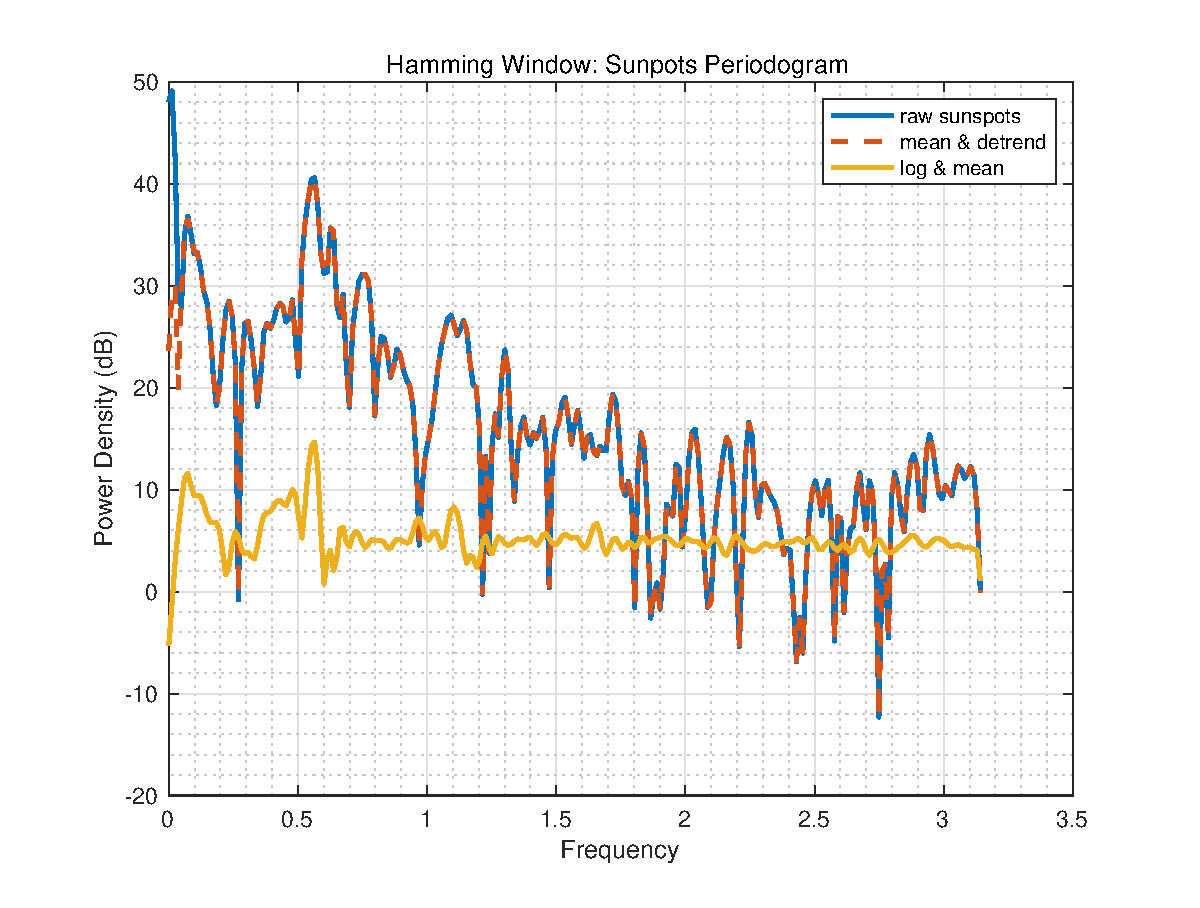
\includegraphics[height=1.5in]{Part1/1_2_a_2.eps}
    \caption{Sunspot time series: Hamming window periodogram method .}
    \label{fig:1_2_a}
\end{figure}
b) Figure \ref{fig:1_2_b_1}, is the standard and Bartlett periodogram of EEG data. The peaks are 8-10 Hz, 13 Hz, 26 Hz, 39 Hz, 50 Hz. The latter plots give the Bartlett method. 
According to the instructions in the booklet, 8-10 Hz is not SSVEP since it is tired while recording.The fundamental harmonic frequency of SSVEP is  at peak of 13 Hz and it is less visible as window length decreased. The first harmonic frequency of SSVEP is at 26 Hz, which is still visible as window length decreased. This may because there is no large interference near it. The second harmonic frequency of SSVEP is at 39 Hz, but it is less visible at lower window lengths. However, 50 Hz is not SSVEP because it has strong power-line-interference even at small window lengths. 

\begin{figure}[H]
    \centering
    \begin{subfigure}{0.35\textwidth}
        \centering
        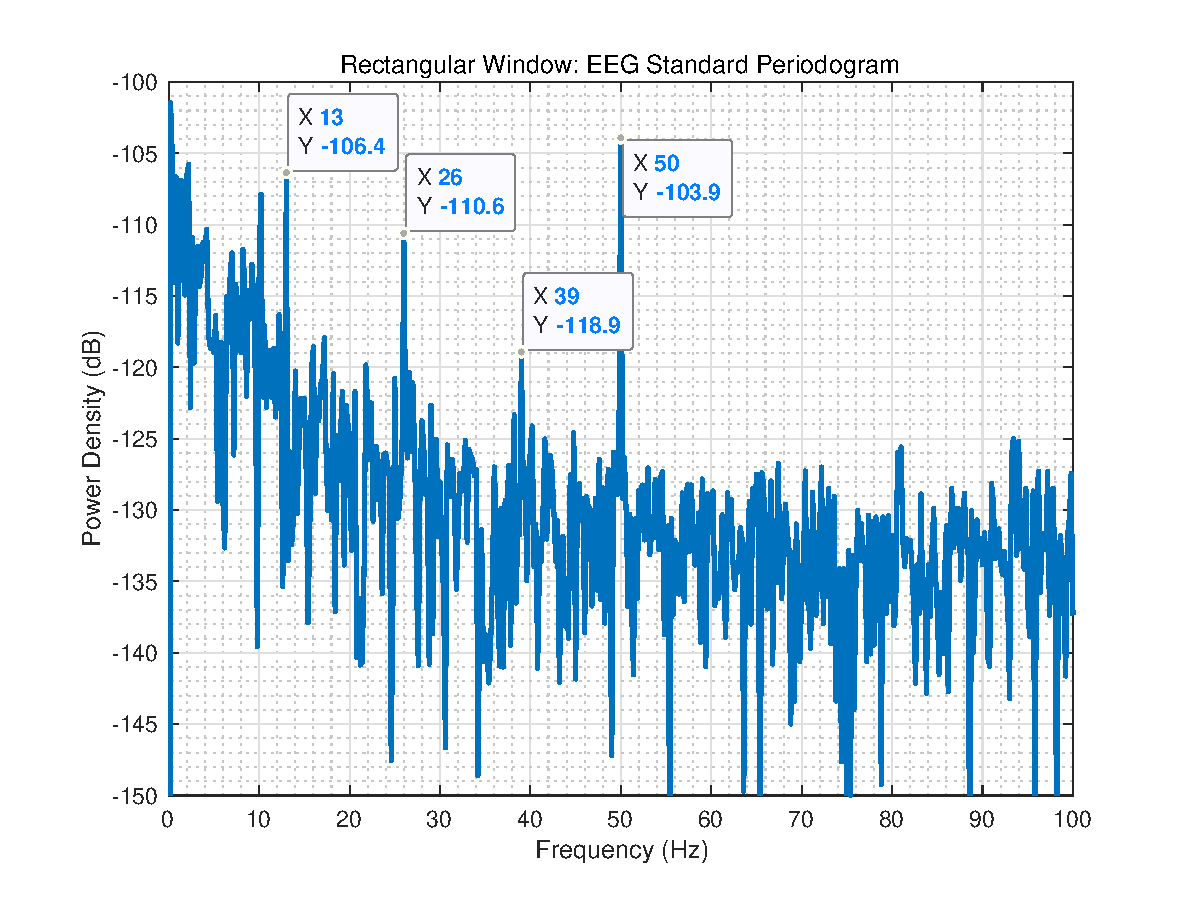
\includegraphics[height=1.5in]{Part1/1_2_b_1.eps}
    \end{subfigure}
    ~ 
    \begin{subfigure}{0.35\textwidth}
        \centering
        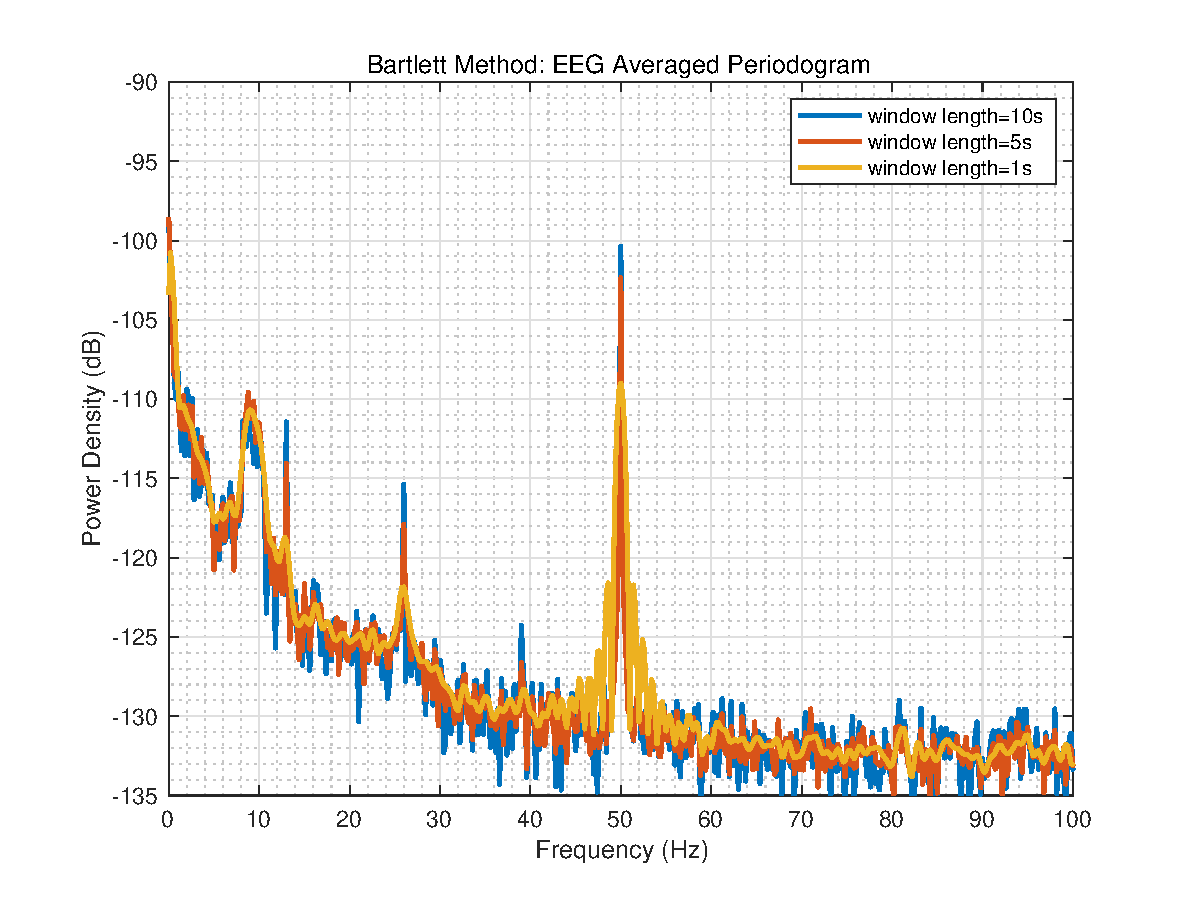
\includegraphics[height=1.5in]{Part1/1_2_b_2.eps}
    \end{subfigure}
    \caption{EEG samples: standard and Bartlett method periodogram with rectangular window .}
    \label{fig:1_2_b_1}
\end{figure}

\ref{fig:1_2_b_2} given the comparison of standard periodogram and averaged periodogram with 10s and 1s window length. It can be seen that as the window lengths become smaller, the components in 8-10 Hz can be still observed adequately.  Theoretically, as window length decreases, the number of captured periodograms increases and the variance decreases. However, the drawback is the frequency resolution also decreases. 
At window length is 10s, it can be seen that, the variance has slightly decreased but the resolution keep unchanged. The later figure with window length 1s, compared with 10s, it has a more reduced variance, but the resolution at peak 39 Hz has lost.
In conclusion, there is a trade-off between frequency resolution and variance minimizing. The situation varies from largest variance and precised resolution for standard periodograms to smallest variance but worst resolution for averaging periodogram with window size only 1s. 
\begin{figure}[H]
    \centering
    \begin{subfigure}{0.35\textwidth}
        \centering
        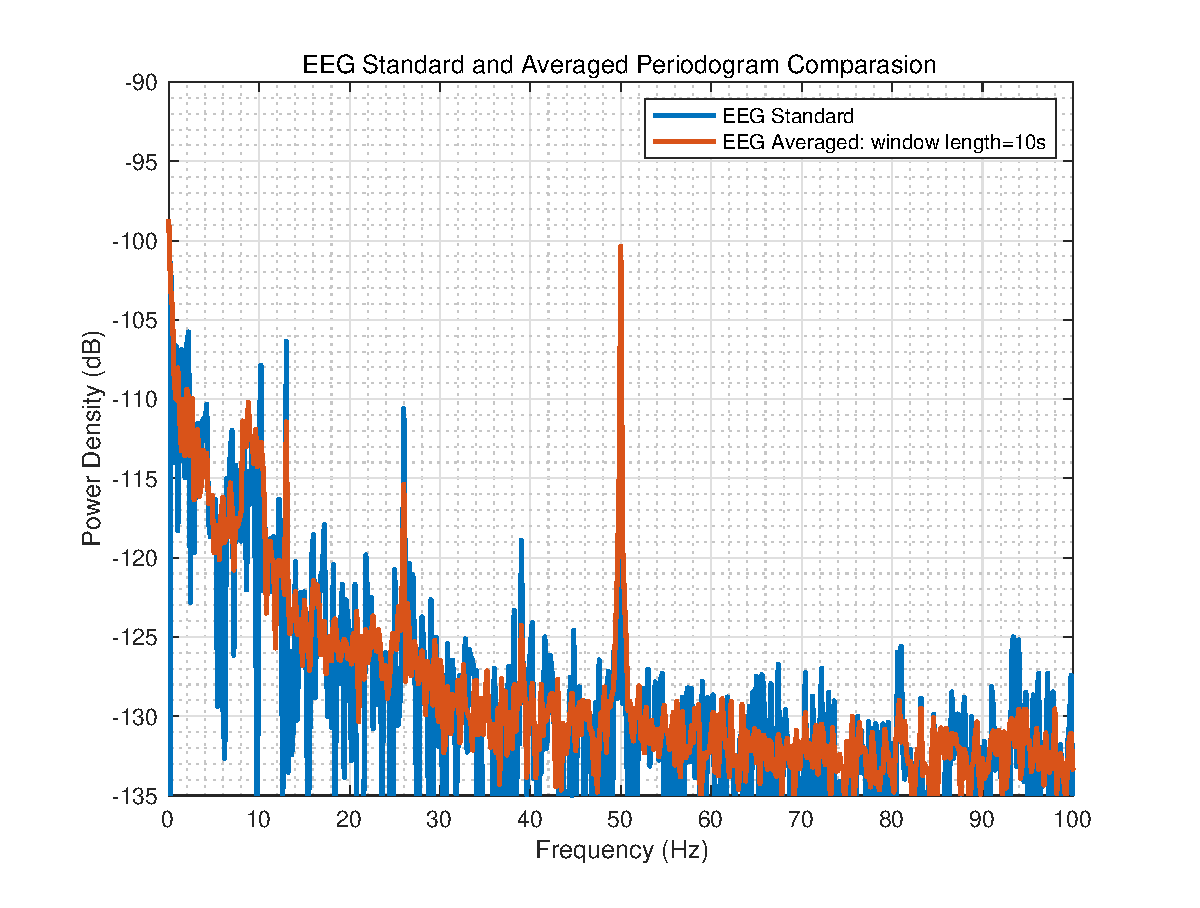
\includegraphics[height=1.5in]{Part1/1_2_b_3.eps}
    \end{subfigure}
    ~ 
    \begin{subfigure}{0.35\textwidth}
        \centering
        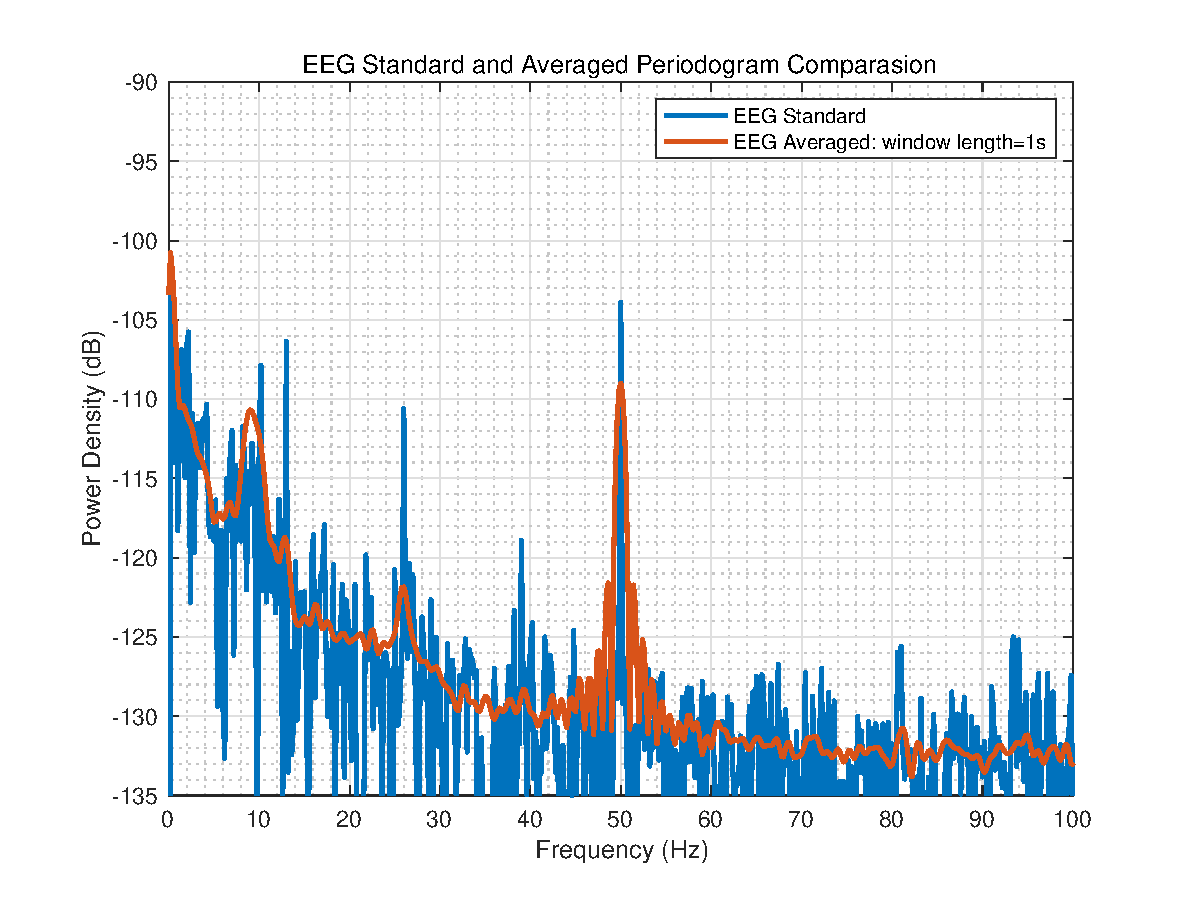
\includegraphics[height=1.5in]{Part1/1_2_b_4.eps}
    \end{subfigure}
    \caption{EEG samples: standard periodogram and averaged  periodogram with of window length 10s and 1s}
    \label{fig:1_2_b_2}
\end{figure}

\section{Correlation Estimation}
a)
Here Figure \ref{fig:1_3_c} shows the biased and unbiased ACF estimation and corresponding correlation for signals like WGN, noisy sinusoidal and filtered WGN. .  
\begin{figure}[H]
    \centering
    \begin{subfigure}{0.35\textwidth}
        \centering
        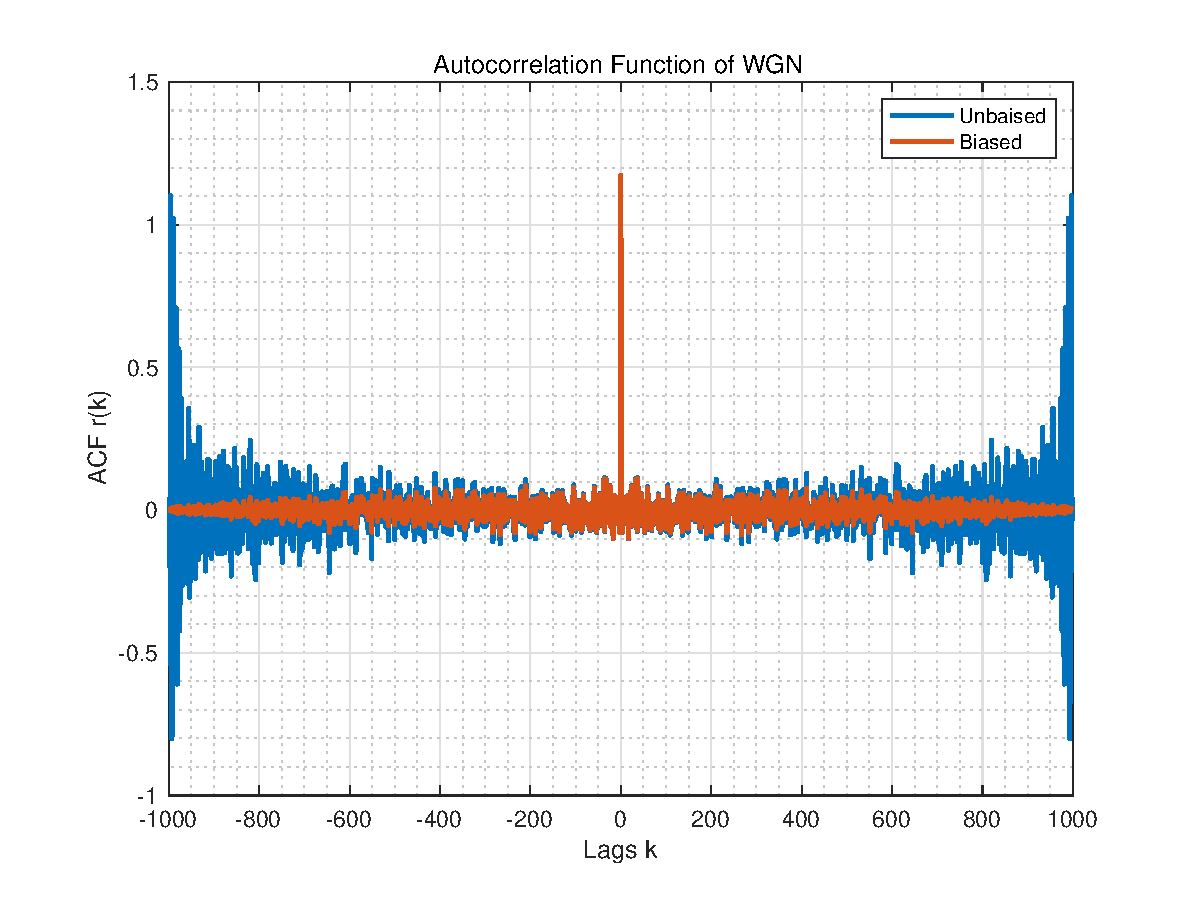
\includegraphics[height=1.5in]{Part1/1_3_a_1.eps}
    \end{subfigure}
    ~
    \begin{subfigure}{0.35\textwidth}
        \centering
        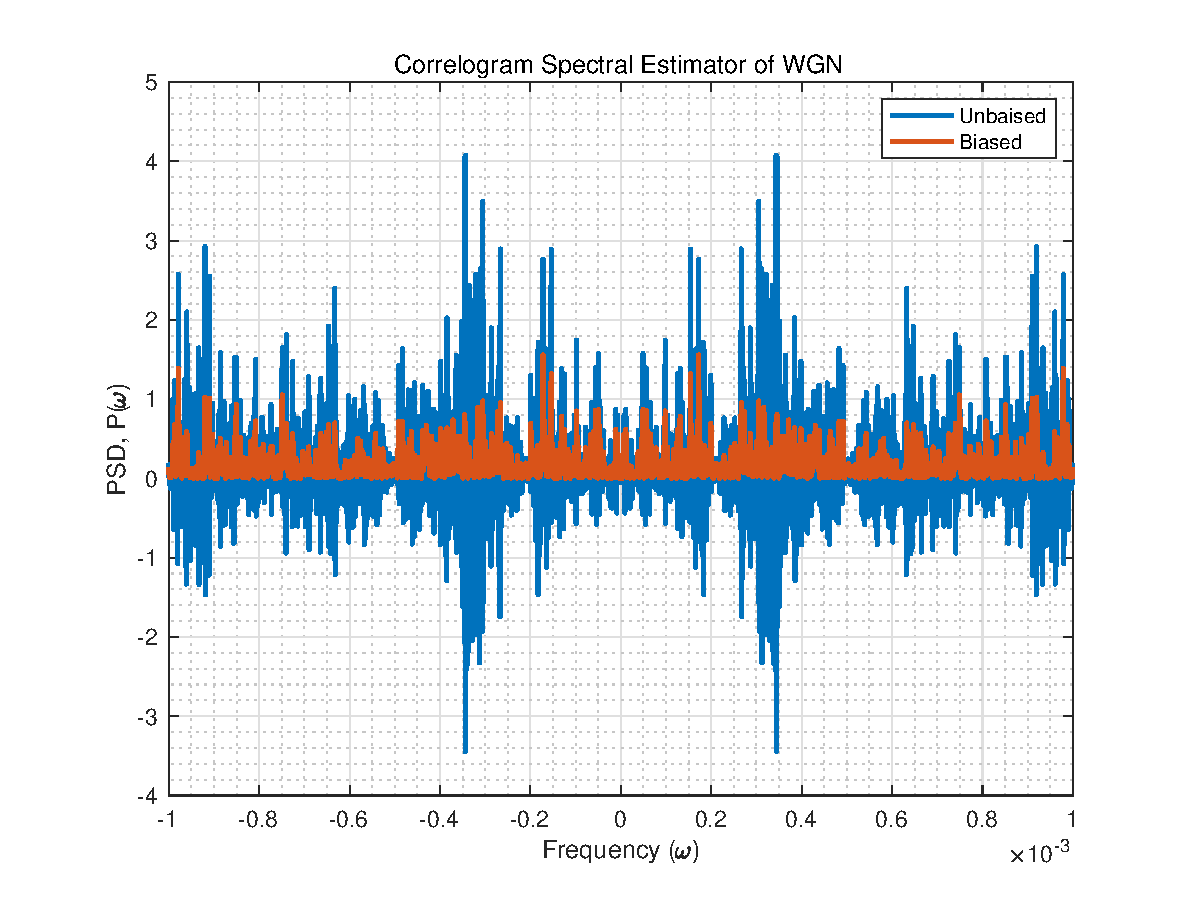
\includegraphics[height=1.5in]{Part1/1_3_a_2.eps}
    \end{subfigure}
    ~
    ~
    \begin{subfigure}{0.35\textwidth}
        \centering
        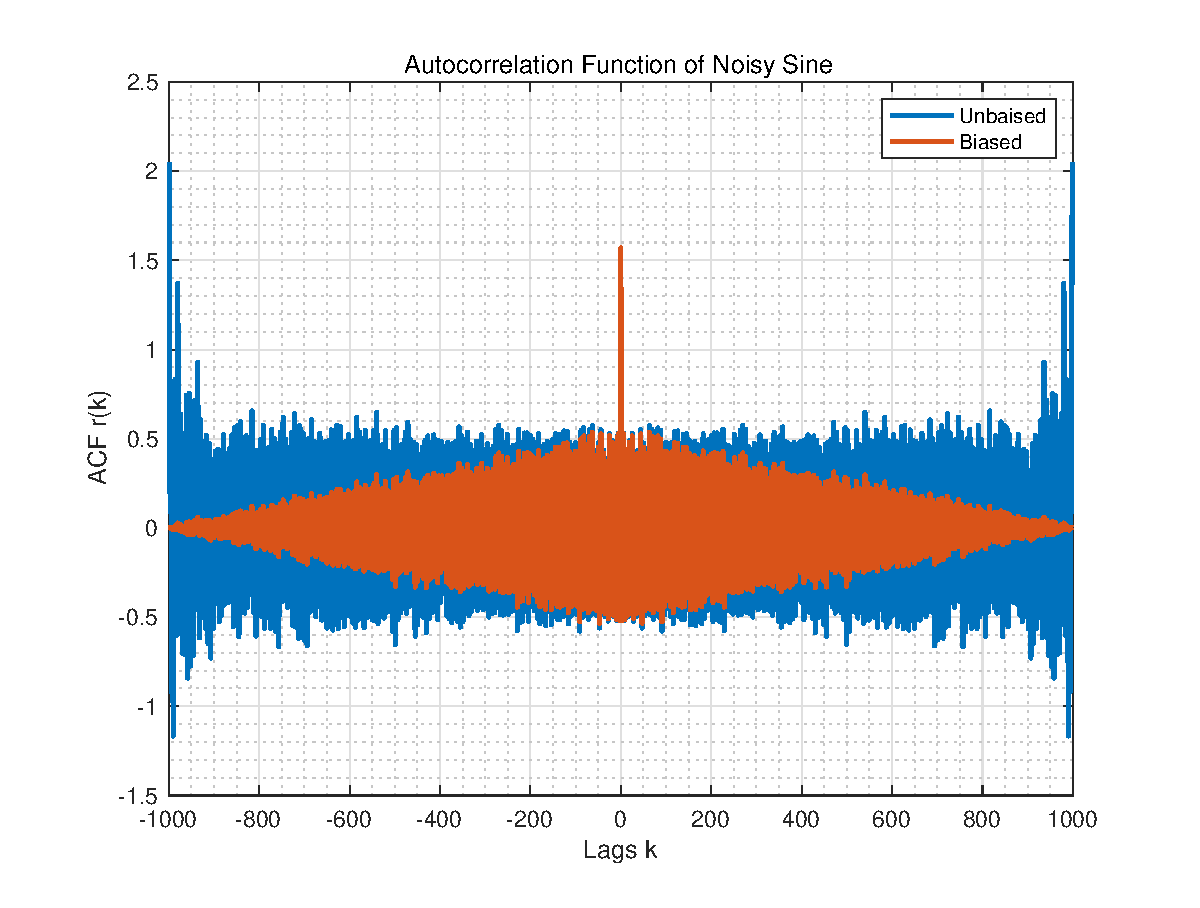
\includegraphics[height=1.5in]{Part1/1_3_a_nosiy1.eps}
    \end{subfigure}
    ~ 
    \begin{subfigure}{0.35\textwidth}
        \centering
        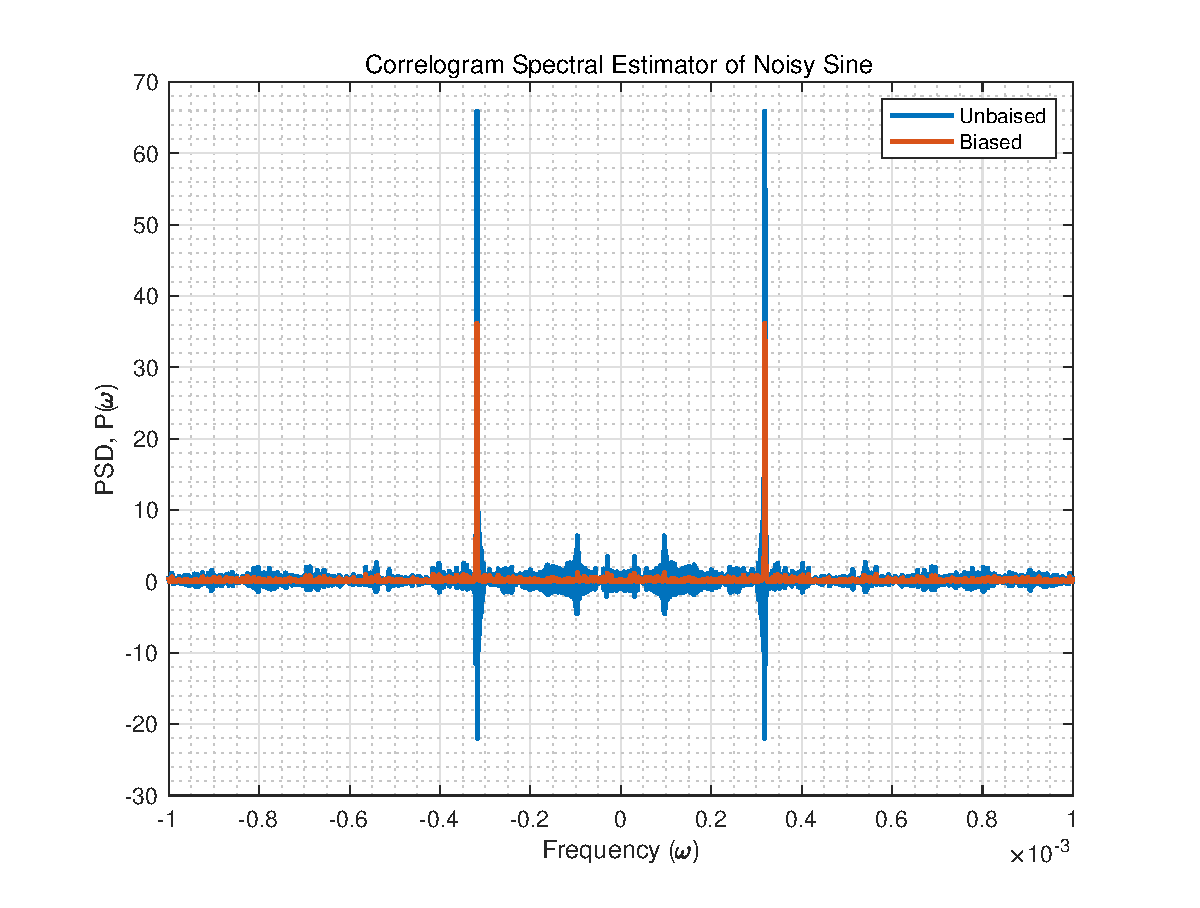
\includegraphics[height=1.5in]{Part1/1_3_a_nosiy2.eps}
    \end{subfigure}
    ~
    ~
    \begin{subfigure}{0.35\textwidth}
        \centering
        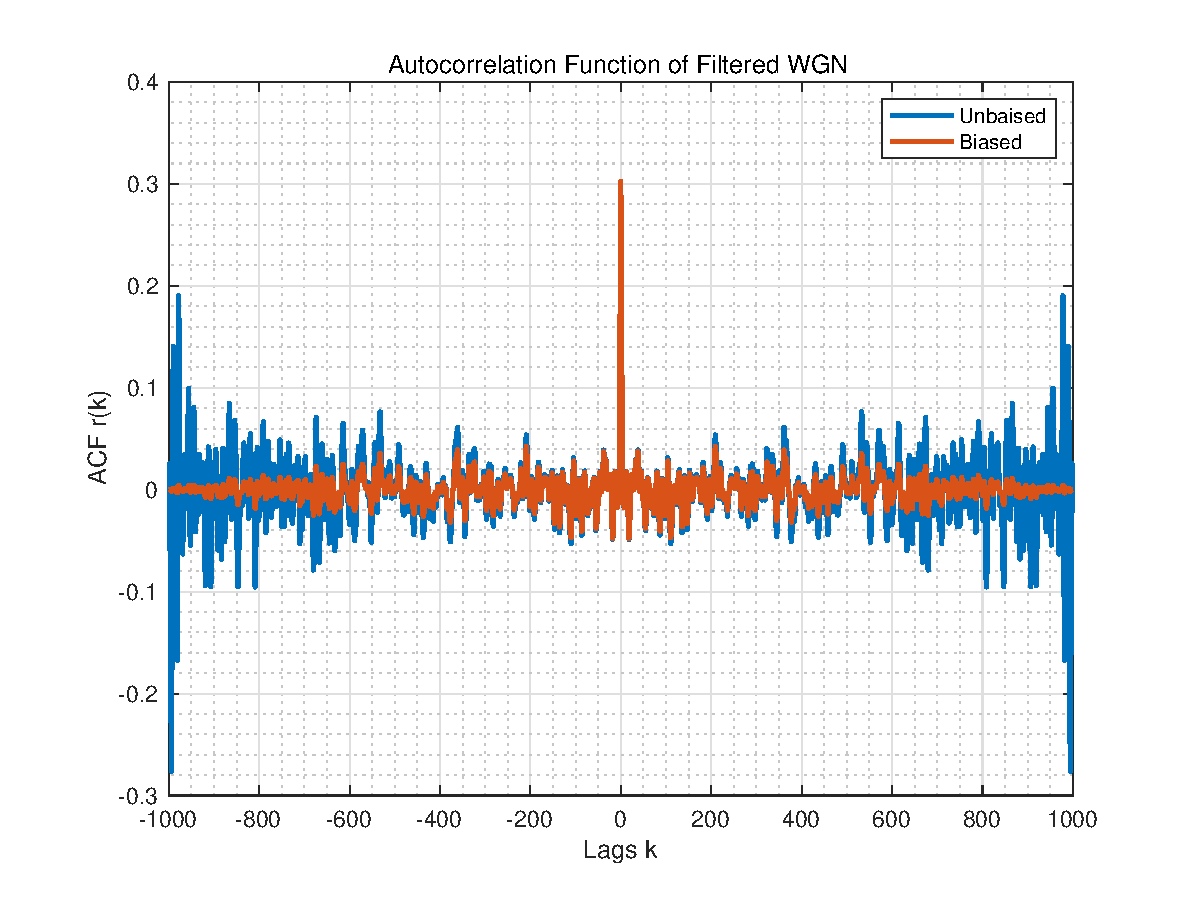
\includegraphics[height=1.5in]{Part1/1_3_a_wgn1.eps}
    \end{subfigure}
    ~
    \begin{subfigure}{0.35\textwidth}
        \centering
        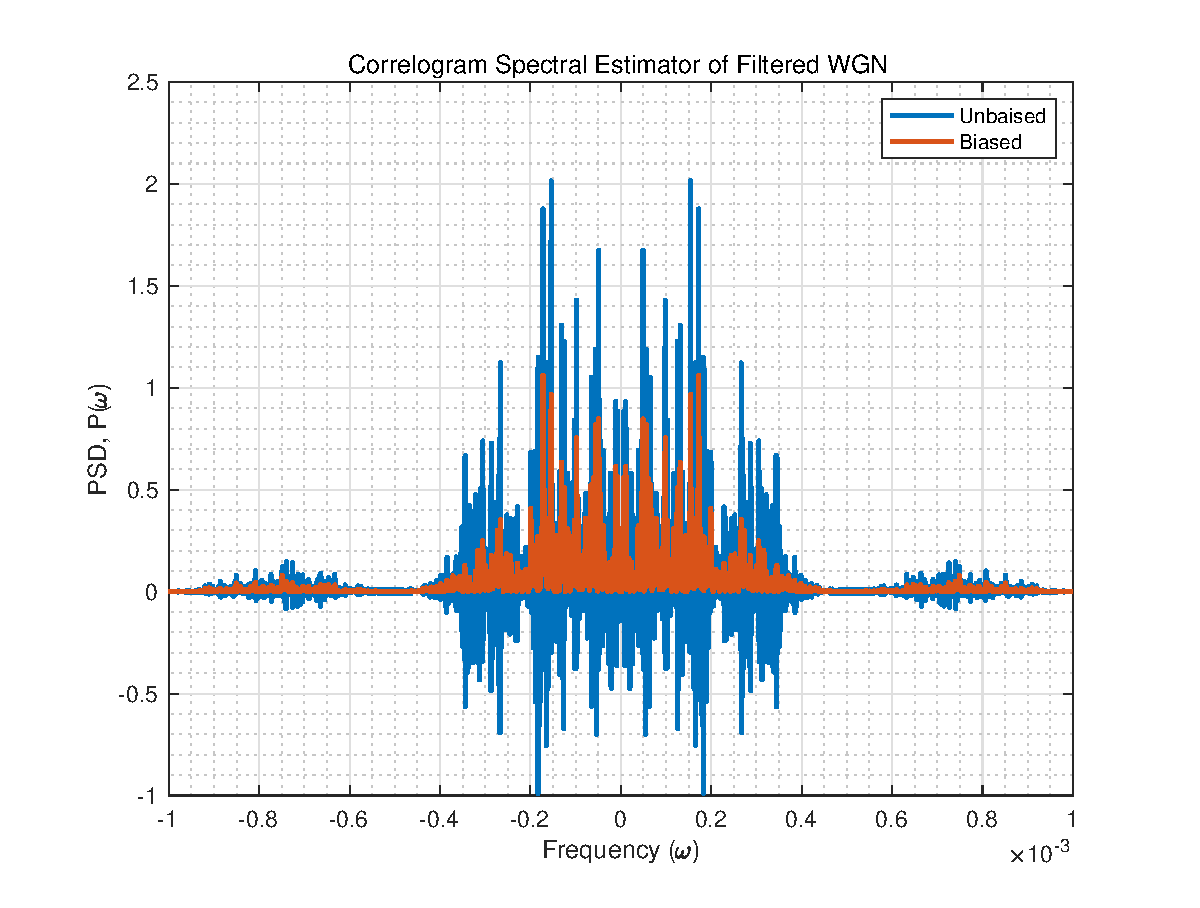
\includegraphics[height=1.5in]{Part1/1_3_a_wgn2.eps}
    \end{subfigure}
    \caption{ACF and Correlogram: biased and unbiased estimates of various signals.}
    \label{fig:1_3_a}
\end{figure}

b)

\begin{figure}[H]
    \centering
    \begin{subfigure}{0.35\textwidth}
        \centering
        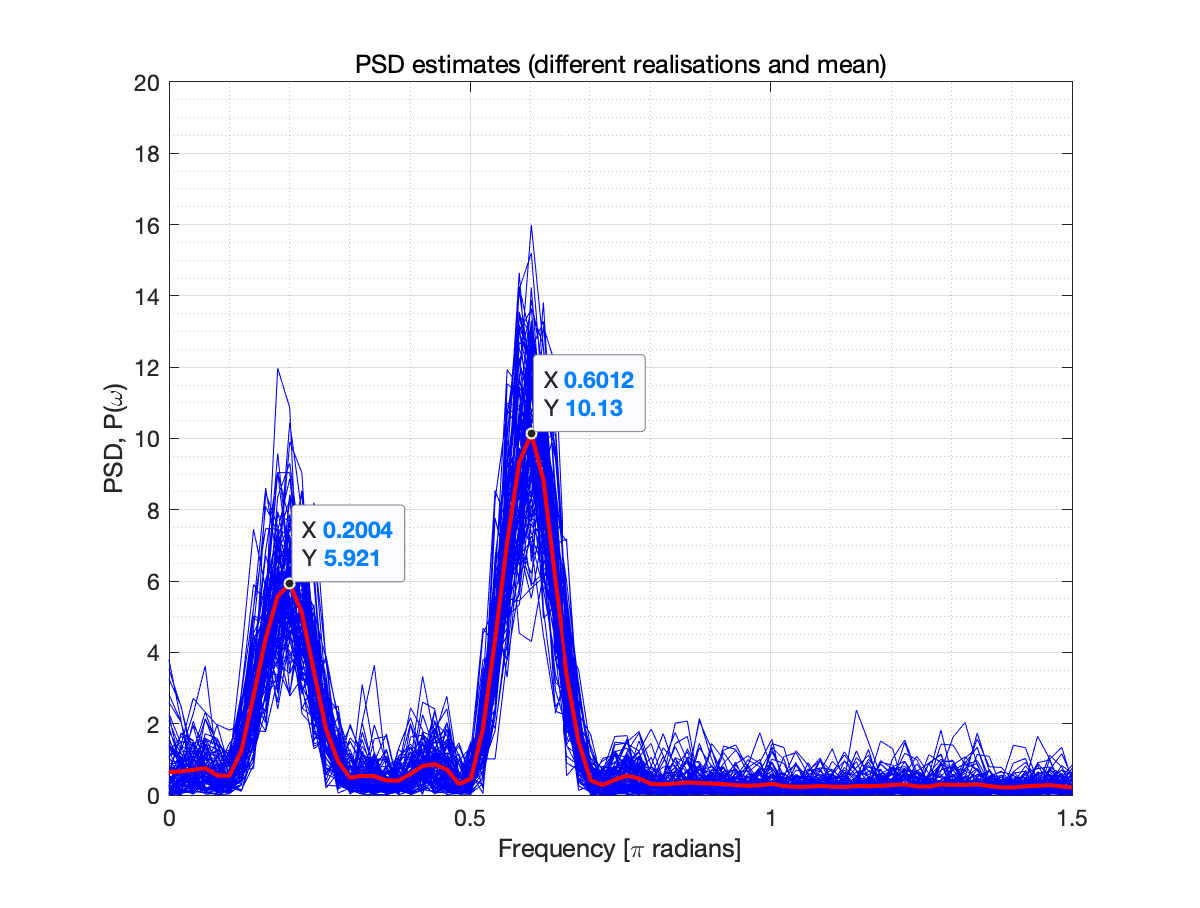
\includegraphics[height=1.5in]{Part1/1_3_b_1.eps}
    \end{subfigure}
    ~ 
    \begin{subfigure}{0.35\textwidth}
        \centering
        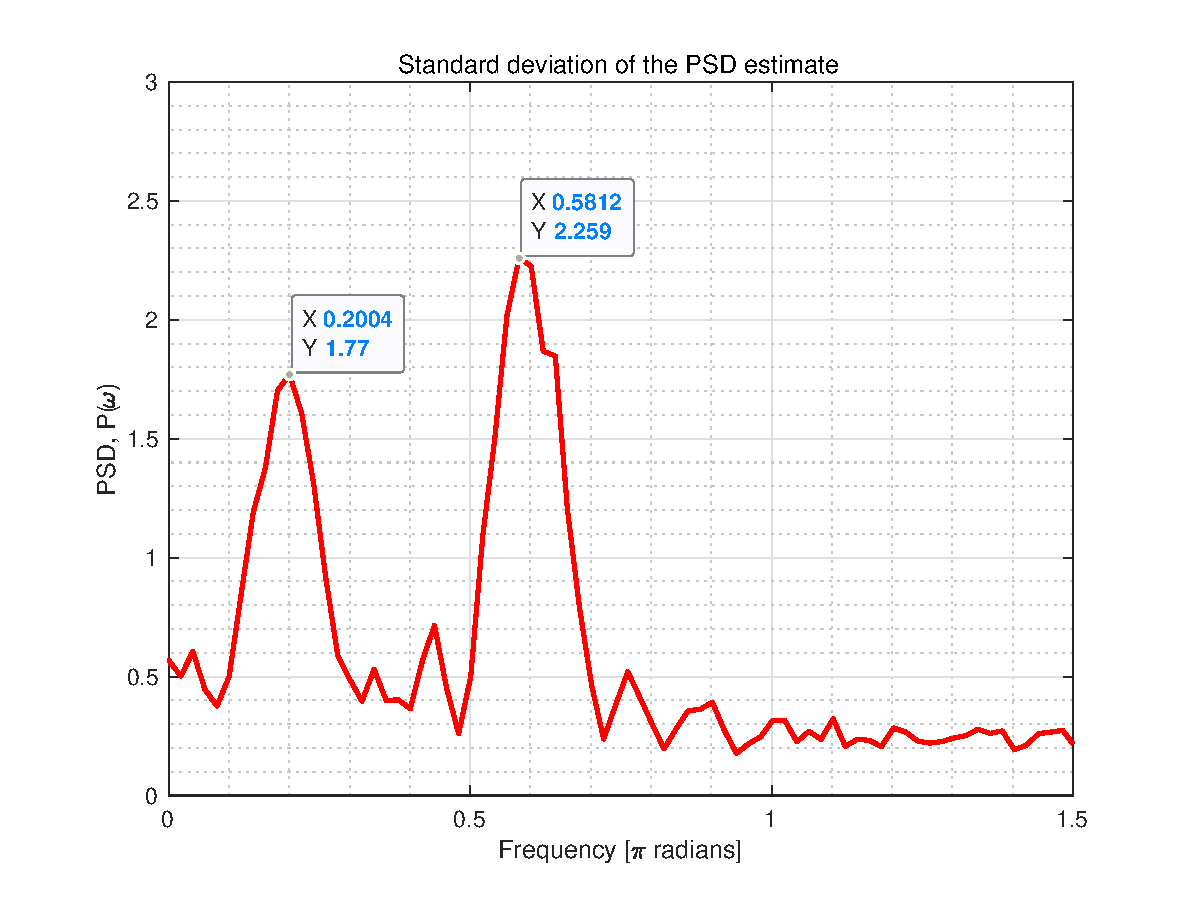
\includegraphics[height=1.5in]{Part1/1_3_b_2.eps}
    \end{subfigure}
    \caption{EEG samples: standard periodogram and averaged  periodogram with of window length 10s and 1s}
    \label{fig:1_2_b_2}
\end{figure}
c)
\begin{figure}[H]
    \centering
    \begin{subfigure}{0.35\textwidth}
        \centering
        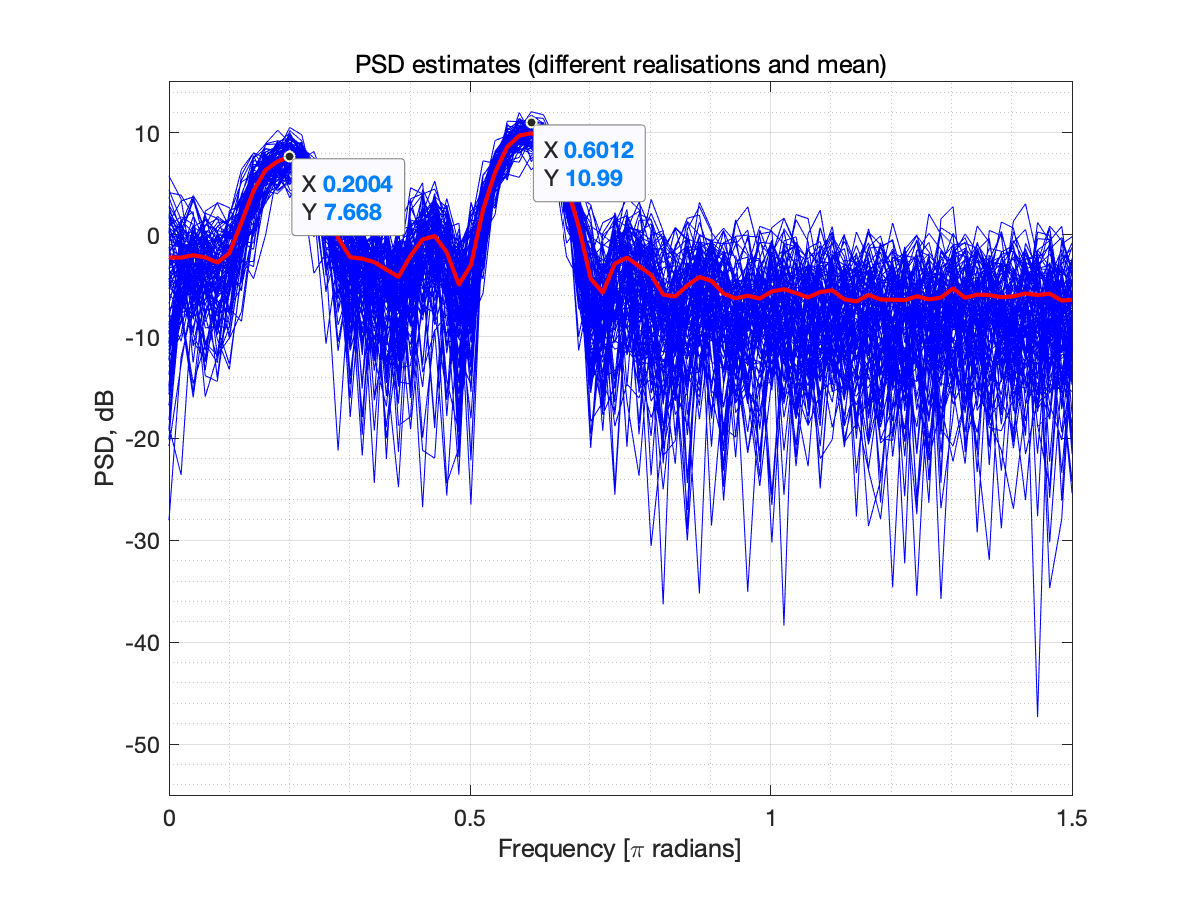
\includegraphics[height=1.5in]{Part1/1_3_c_1.eps}
    \end{subfigure}
    ~ 
    \begin{subfigure}{0.35\textwidth}
        \centering
        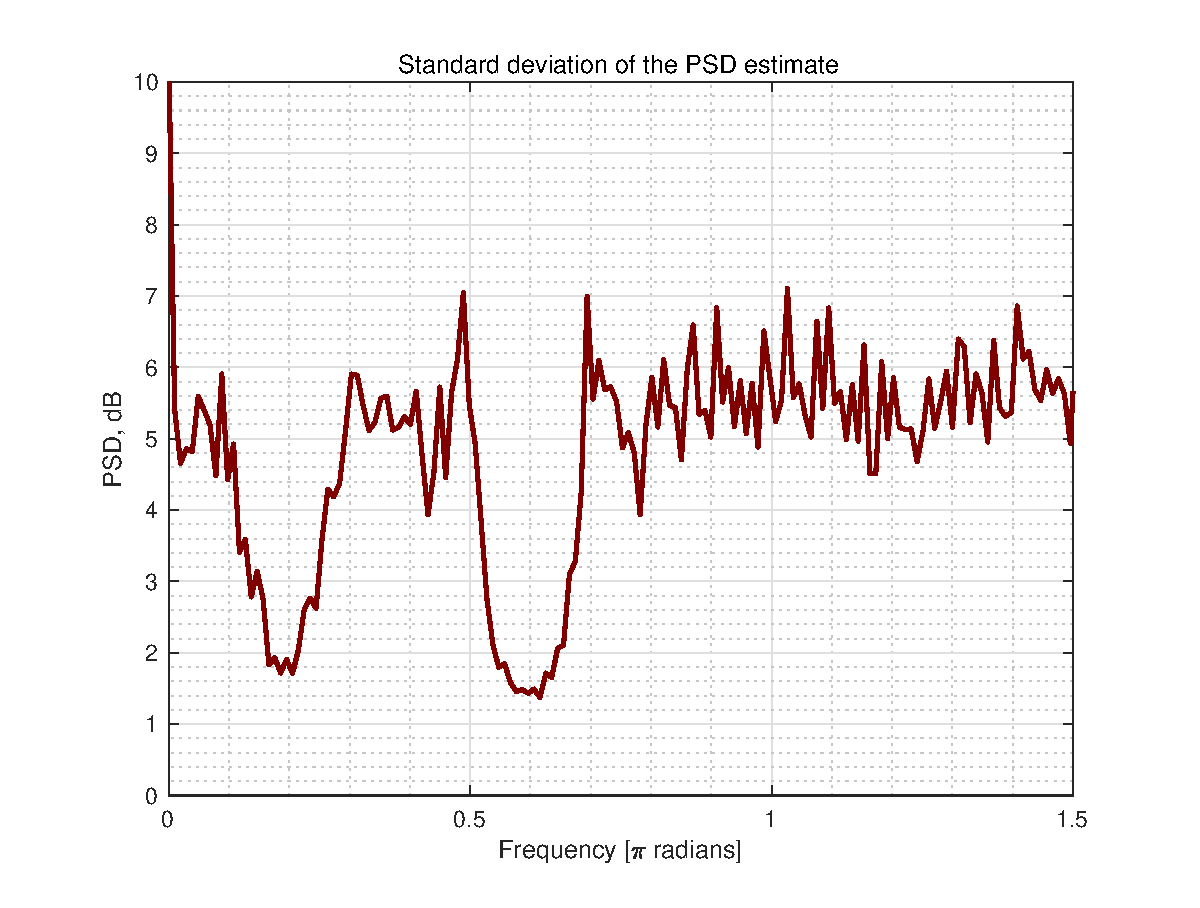
\includegraphics[height=1.5in]{Part1/1_3_c_2.eps}
    \end{subfigure}
    \caption{EEG samples: standard periodogram and averaged  periodogram with of window length 10s and 1s}
    \label{fig:1_3_c}
\end{figure}
d)

\begin{figure}[H]
    \centering
    \begin{subfigure}{0.35\textwidth}
        \centering
        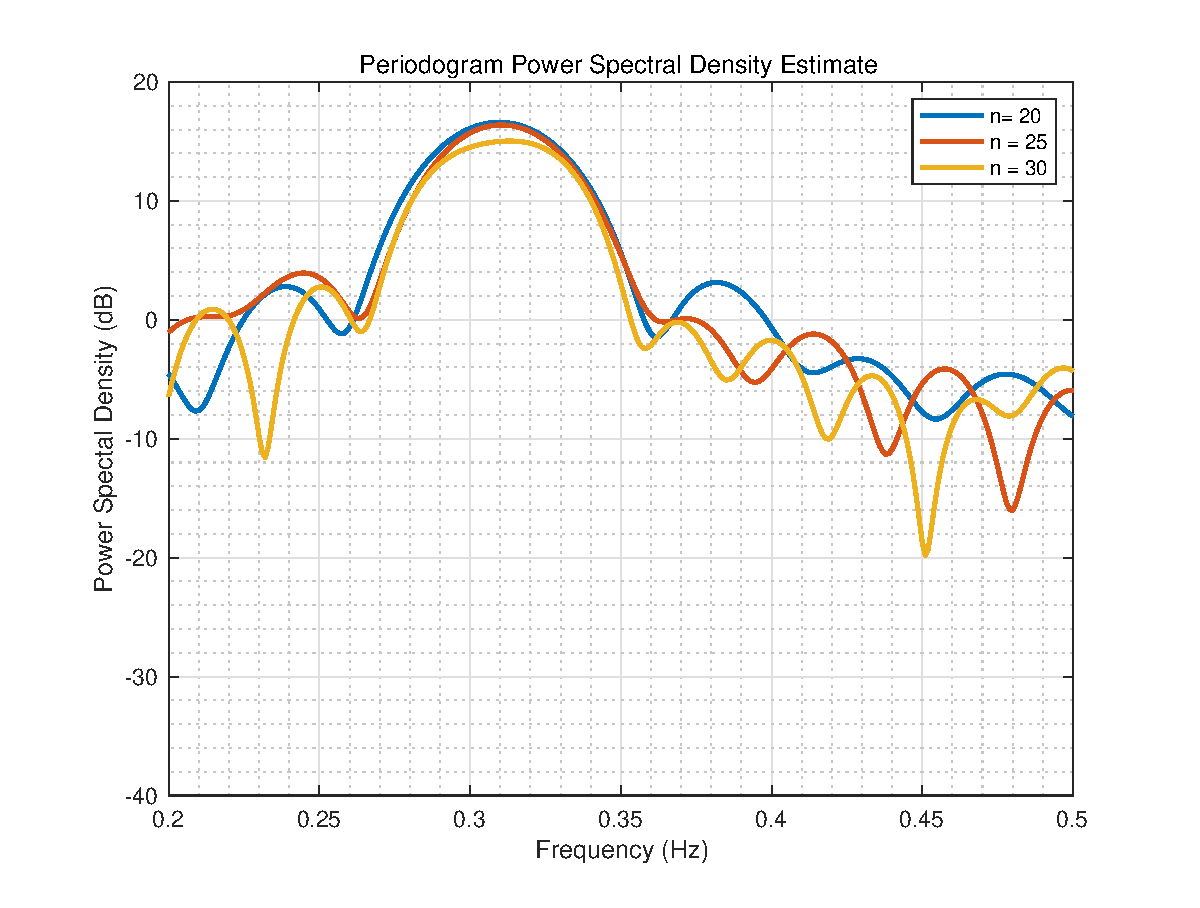
\includegraphics[height=1.5in]{Part1/1_3_d1.eps}
    \end{subfigure}
    ~ 
    \begin{subfigure}{0.35\textwidth}
        \centering
        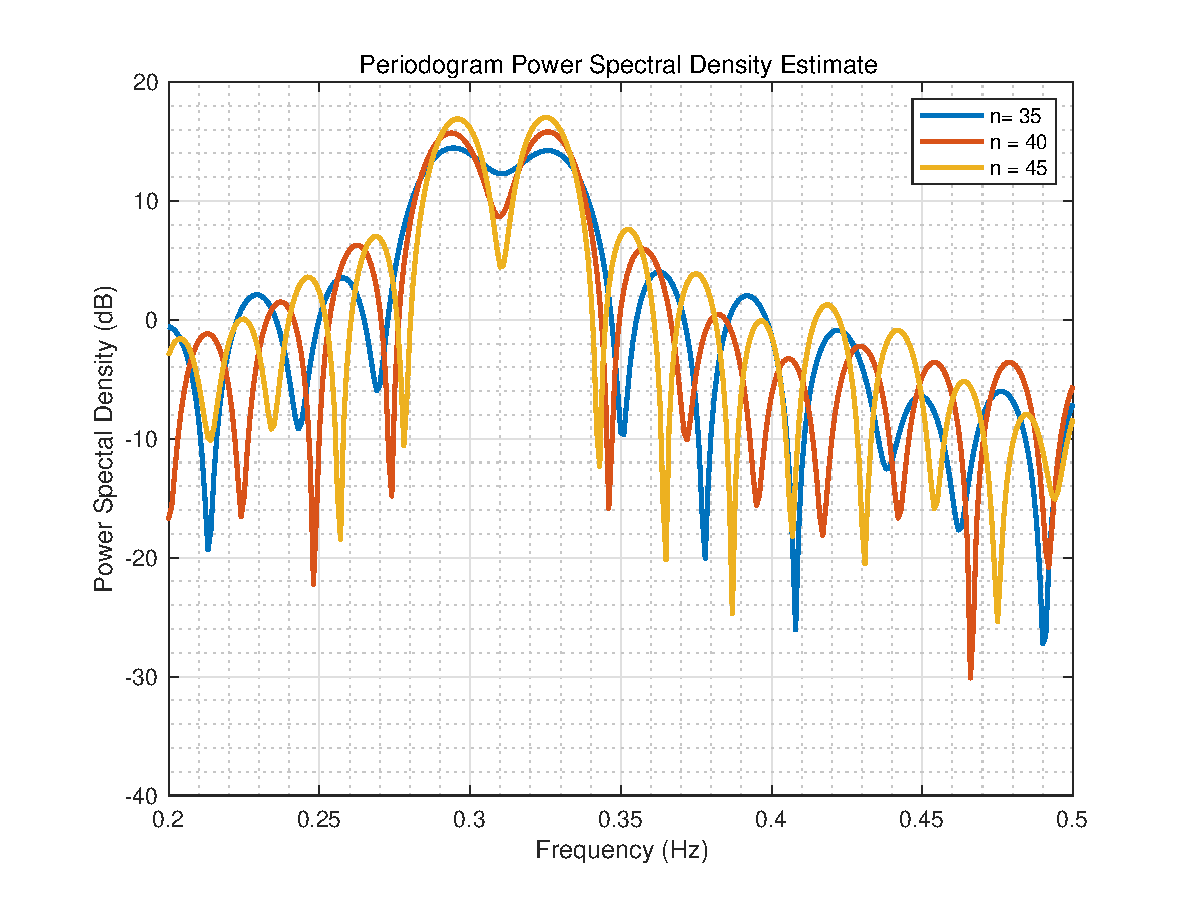
\includegraphics[height=1.5in]{Part1/1_3_d2.eps}
    \end{subfigure}
    \caption{EEG samples: standard periodogram and averaged  periodogram with of window length 10s and 1s}
    \label{fig:1_3_d_1}
\end{figure}
\begin{figure}[H]
    \centering
        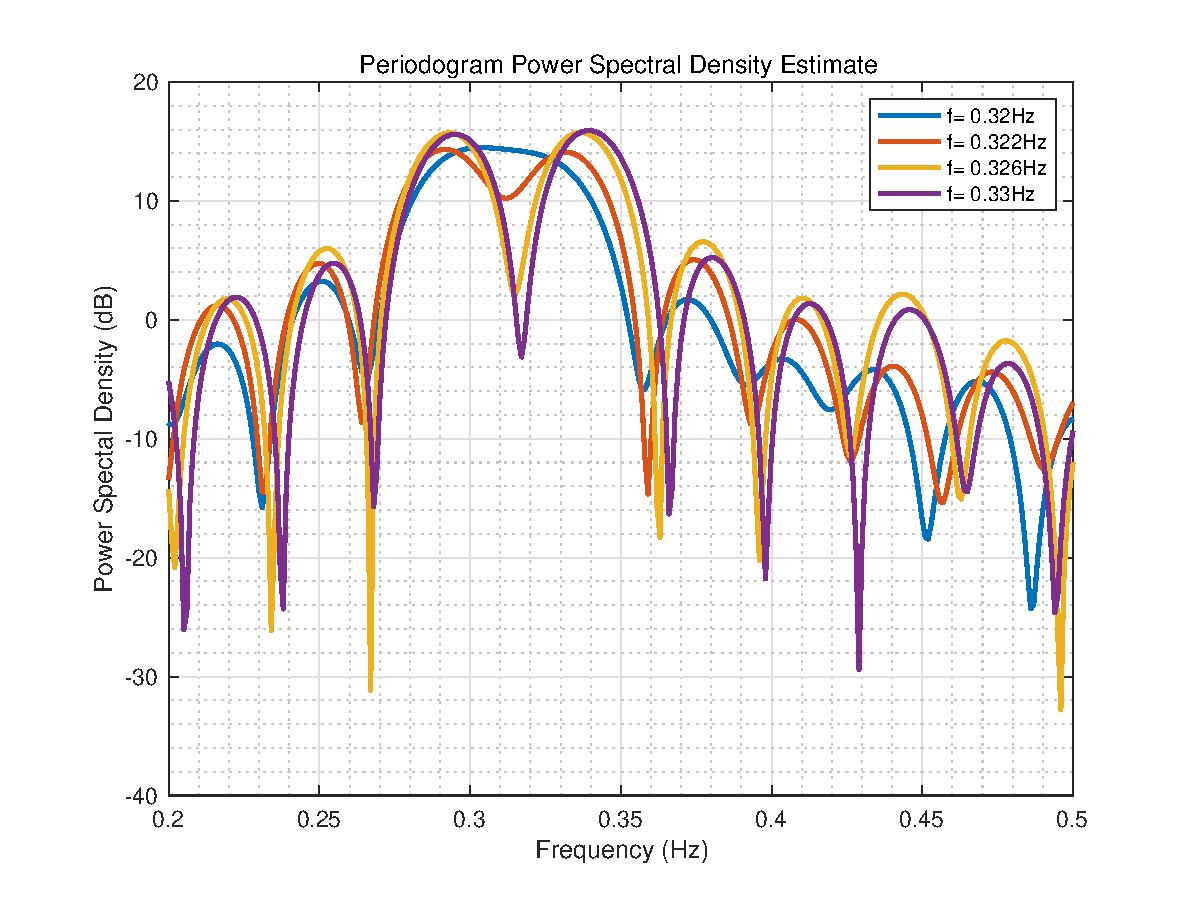
\includegraphics[height=1.5in]{Part1/1_3_d3.eps}
    \caption{Sunspot time series: Hamming window periodogram method .}
    \label{fig:1_3_d2}
\end{figure}
e)
\section{Spectrum of Autoregressive Processes}
%%a)
%% b)
%
\section{Real World Signals: Respiratory Sinus Arrhythmia from RR-Intervals}

\section{Robust Regression}

